%!TEX root = ../template.tex
%%%%%%%%%%%%%%%%%%%%%%%%%%%%%%%%%%%%%%%%%%%%%%%%%%%%%%%%%%%%%%%%%%%
%% sdvn.tex
%% NOVA thesis document file
%%
%% Chapter with introduction
%%%%%%%%%%%%%%%%%%%%%%%%%%%%%%%%%%%%%%%%%%%%%%%%%%%%%%%%%%%%%%%%%%%

\typeout{NT FILE sdvn.tex}%

\chapter[Software Defined Vehicular Network]{\gls{sdvn}}
\label{cha:sdvn}

% Introduction
The \gls{sdn} paradigm has been identified by some researchers and other experts as a powerful and promising tool for addressing some of the challenges posed by \glspl{vanet}\cite{smida_efficient_2020}. As previously discussed, \gls{sdn} is a methodology rather than a specific technology, which allows it to be applied to \glspl{vanet}. This line of thought created a new networking paradigm that is primarily known as \gls{sdvn}, although the term \gls{sdvanet} is also occasionally used.

The concept of \gls{sdvn} was first introduced by Ku et al. in \cite{ku_towards_2014}, and since then there have been many different proposals of how to implement the \gls{sdn} principles in \glspl{vanet}. \gls{sdvn} has recently received significant support from researchers, which has resulted in significant technical and architectural advances in \gls{sdn}-enabled vehicular networks\cite{bhatia_software_2019}. 

Similarly to traditional wired networks, non-\gls{sdn} systems function reasonably well. Therefore, the implementation of \gls{sdn} should not be seen as a solution to make \glspl{vanet} work, but rather as a means to enhance them.

% Benefits/Challenges
\section{Benefits and Challenges}

The implementation of the \gls{sdn} paradigm in \glspl{vanet} is driven by the desire to bring some of the improvements of \gls{sdn} to \glspl{vanet} to tackle the challenging requirements of \glspl{vanet}. This paradigm has the potential to introduce flexibility, programmability, and centralized control to vehicular networks\cite{bhatia_software_2019}. This section reflects upon the benefits of \gls{sdn} and the characteristics of \glspl{vanet} to extrapolate the benefits and possible challenges that \gls{sdvn} can offer today.

% Mandated Interoperability
\subsection{Mandated Interoperability}

As previously stated in Section \ref{sec:Applications_of_VANETs}, \glspl{vanet} require high road acceptance for their useful applications to be effective. This implies that all implemented devices must be able to communicate with each other, and to this end the EU has tried to standardize devices to promote interoperability between different vehicle manufacturers.

In \gls{sdn} networks, operators have complete control over a static network, making it easy to conceal the inner workings of devices from the rest of the Internet and implement them as desired. However, in \gls{sdvn} the same is not possible because a vehicle \gls{its} subsystem must be able to communicate with every single roadside \gls{its} station in order to access infrastructure services deployed in the central \gls{its} subsystem. \gls{sdvn} devices must be compliant with existing regulation and communicate with standardized protocols in order to be interoperable with other devices.

% Higher network control 
Such an emphasis on interoperability undermines the powerful control that \gls{sdn} brings. Network operators and developers can't take full advantage of the freedom this technology provides to implement new algorithms and test them in real-world scenarios. Even the effectiveness of the additional control provided by P4 is reduced by the inability to change network protocols.

This is not to say that the increased control that \gls{sdn} brings is completely useless, as it can still provide some advantages in dealing with certain scenarios, but this \gls{vanet} characteristic largely limits what can be accomplished with \gls{sdn}. 

It is also relevant to note one of the major goals of \gls{sdn}, which is to move network control from manufacturers to operators, with the ultimate goal of giving it to network users. In vehicular networks, the identity of the network operator becomes an implementation detail, but it will most likely be the same government of private entities deploying the infrastructure. \gls{sdn} continues to provide these operators with greater network control, but it cannot be given to users for fear of being misused for nefarious purposes.

% Network innovation
\subsection{Network innovation}

Another important conclusion to be drawn from the above is that the technologies that will form future \glspl{vanet} can be expected to be even more static than in traditional wired networks. On top of that, current hardware defined devices exacerbate this problem, as any fundamental change to \glspl{vanet} would require the hardware of thousands of roadside systems and millions of vehicle systems to be manually replaced. This presents a logistical nightmare, making it highly unlikely that this scenario would happen except in the rarest of cases, and then only if mandated by the EU. This reality is evidenced by the slow and arduous standardization process that \glspl{vanet} have undergone over the last 20 years, which has sought to find a single solution for \glspl{vanet} that would act as a definitive and permanent answer to all of its problems. 

\gls{sdvn} allows new functionalities to be implemented in the same hardware through software updates, facilitating changes to be made throughout the network. This could considerably accelerate the adoption of this technology and facilitate the implementation of any future fix or optimization.

% Network management and performance improvements
\subsection{Network management and performance improvements}

Even more than in static networks, \gls{sdn} can provide \glspl{vanet} with more flexible and intelligent packet flows, channel allocation, and connectivity. Traditional \gls{vanet} routing algorithms are limited to the individual perception of each node as they are implemented in each individual device. \gls{sdn} is built on a global view to make better decisions based on the combined information from multiple sources, which results in better network performance since informed decisions lead to more optimal outcomes. The automated network capabilities brought about by \gls{sdn} also have the potential to address \gls{vanet}'s adversities. Listed below are some of the characteristics of a \gls{vanet} and how they can be enhanced through the implementation of \gls{sdn}.

\begin{description}
    % include \ref{subsec:predicted_mob} refs to all characteristics?
    % High mobility
    \item[High mobility] In an environment where topology changes occur frequently, it is critical to be capable of adapting to sudden and unexpected events. \gls{sdn} provides flexibility, which allows for more dynamic network configuration, enhancing the network's responsiveness to emergencies and changing requirements, while also enabling it to better adapt to changing conditions and needs\cite{ku_towards_2014}.
    % Predictable mobility
    \item[Predictable mobility] \gls{sdvn} can leverage the centralized view of the network, to better exploit the predictable mobility when compared to traditional approaches. The controller can use a vehicle's information to predict future topology changes and set traffic rules accordingly, improving connectivity and overall network performance.  
    % Congestion and scalability issues
    \item[Congestion and scalability] Network congestion and the variable vehicle density are issues that can be reduced by leveraging the global view of the network to better optimize the available mediums. Centralizing network control increases cooperation, allowing the optimal path to be calculated, which reduces delays and overhead\cite{smida_efficient_2020}. Also, situations of high vehicle density can be more easily predicted and the transmission power levels on vehicles can be jointly adjusted based on future vehicle network density, greatly reducing interference\cite{smida_efficient_2020}. Overall, automated tools promise to make run-time changes to networks based on the unique characteristics of \glspl{vanet}, helping to achieve a better performing network.
\end{description}

% Issues with maintaining a global network view
\subsection{Issues with maintaining a global network view}

The advantages of centralized control are plentiful, but the establishment of this centralized view in \gls{vanet} is not guaranteed. \glspl{vanet} are based on wireless connectivity, which causes the southbound API to suffer from instability and even complete unavailability\cite{cardona_software-defined_2020}. Combined with volatile topologies, this results in increased communication delays in the southbound interface, which can lead to inaccuracies in the controller's view of the network and in the rules established in the switches, casting doubt on the controller's ability to maintain an accurate and up-to-date view of the global topology\cite{ben_jaballah_security_2020}. 

Another major concern introduced with \gls{sdvn} is the management overhead introduced by the southbound API required for the controller to manipulate the devices, as switches must be frequently updated to accurately reflect the network's state. This could result in additional traffic and increased network congestion compared to the distributed methods used in traditional networks.

At the same time, it should be noted that it may not be necessary for all instances of the controller to maintain a global view of the entire network. Instead, individual instances of the controller may only need to keep track of a small region of the network, as most messages in \glspl{vanet} are only relevant in their immediate surroundings\cite{sarpong_potential_2023}.

In summary, the dynamic state of the network combined with poor controller connectivity presents a major concern in \gls{sdvn}. The process of maintaining an updated view of the global network topology becomes costly and time-consuming due to potential inaccuracies in the updated information\cite{ben_jaballah_security_2020}. To address this issue, it is important to ensure robust protection against loss of connectivity and to guarantee the availability of the control plane, which sometimes requires the integration of other technologies such as fog computing with \gls{sdn}\cite{ben_jaballah_security_2020}.

% cheaper networks
\subsection{Cheaper networks}

When considering the deployment of \gls{vanet} technology, the cost of infrastructure is a major concern, with up to 86\% of the total expected cost being attributed to hardware\cite{asselin-miller_study_2016}. Just as in traditional networks, \gls{sdn} can reduce costs by reducing complexity and increasing modularity while promoting interoperability.

% Security
\subsection{Network security}

The introduction of the \gls{sdn} paradigm does not introduce any new significant security or privacy challenge to \glspl{vanet}. Some researchers\cite{ben_jaballah_security_2020} mention the centralized controller as a new vulnerability that can be exploited, but in reality current \gls{vanet} deployment already relies on services provided by the central \gls{its} subsystem.

% Architecture 
\section[SDVN architecture]{\gls{sdvn} architecture}

The \gls{sdvn} architecture can be represented based on either of the architectures of the two technologies that define it. Of the two, the most suitable is the architecture of \gls{sdn}. The \gls{vanet} architecture is best represented by the \gls{its} host architecture, which is built on the OSI model. The \gls{sdn} paradigm aims to move the internet away from closed and complex standardized protocols and into open and simple network components. As such, the \gls{sdvn} architecture inherits the format as the general \gls{sdn} architecture, retaining the three layers present in it as can be seen in Figura \ref{fig:sdvn_arciotecture}. 

\begin{figure}
	\centering
	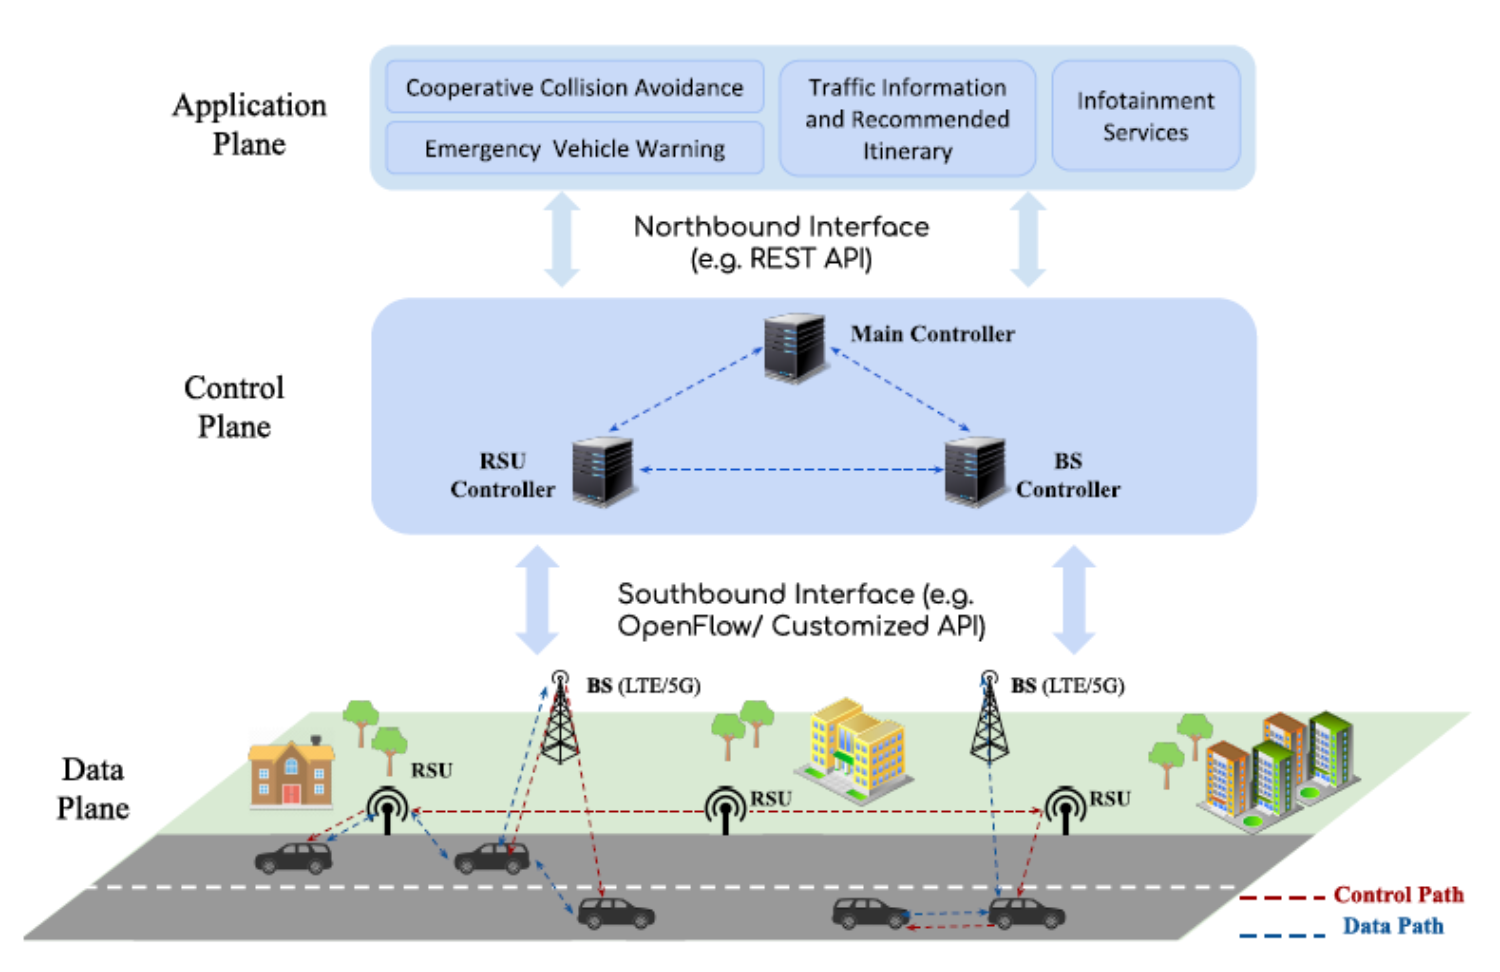
\includegraphics[width=0.8\textwidth]{Chapters/Figures/SDVNs/architecture.png}
	\caption{Conceptual view of \gls{sdvn} architecture\cite{toufga_towards_2020}}
	\label{fig:sdvn_arciotecture}
\end{figure}

	% Data plane
\subsection{Data plane}

In \gls{sdvn}, as in \gls{sdn}, the data plane consists of all forwarding hardware but these components can be divided into two different categories based on whether they are wired or wireless. Mobile hardware refers to the vehicle \gls{its} station, while stationary hardware refers to the routers and switches found in the remaining \gls{its} subsystem. Network intelligence is extracted from all \gls{its} stations, but due to the special characteristics of the mobile nodes all \gls{sdn} enabled devices cannot be treated the same. 

	% Control plane
\subsection{Control plane}

The control plane remains almost unchanged as the centralized logical intelligence of the network, managing device behavior to achieve desired policies. It remains responsible for communicating the high-level applications defined in the application plane to the devices in the data plane, and for transmitting device information from the data plane to the application plane. The main difference introduced by \gls{sdvn} is a consequence of the need to manage devices in the ad hoc space. Due to the two distinct types of components in the data plane, unique and customized networking applications are required to address the unique nature of each scenario. Managing the wired portion of the network can be considered a simple task because the process is the same as \gls{sdn}, whilst the wireless domain presents unique challenges and requires distinct solutions to manage wireless resources as effectively as wired resources\cite{cardona_software-defined_2020}.

In \gls{sdvn} controller distribution becomes a central concern. Vehicular networks have immense coverage given that they include all roads, and due to this vast distribution, a single controller cannot handle the traffic of the entire network. Therefore, it is out of the question for scalability and delay reasons\cite{toufga_openflow_2018}. Instead, the control plane must consist of multiple physical controllers efficiently distributed across the network, coordinating their decision-making efforts to handle the high volume of traffic\cite{ben_jaballah_security_2020}. Another important motivation for distributing the control plane is to bring the controller closer to the vehicles to reduce communication delays between the data and control planes\cite{nkenyereye_software-defined_2019}. 

It should be noted that a truly distributed controller, where all instances have global information of the network, seems impossible and even counterproductive. To perform effectively, controllers usually only need information about a specific part of the network, which is in part because some messages are only relevant in the context of that particular section of the network\cite{cardona_software-defined_2020} and the ones that aren't should be directed to the nearest roadside \gls{its} station. The size and the transition between regions is dependent on implementation. 

That being said, there exist many different controller placement distributions proposed in the literature. In practice, the controller can be located in the central, roadside, or vehicle subsystems. Different architectures place the controllers in a combination of these stations, giving them distinct responsibilities and utilizing different methods to distribute intelligence between them.

Most approaches to controller distribution in the literature\cite{bhatia_software_2019}\cite{cardona_software-defined_2020}\cite{toufga_openflow_2018} converge on a two-tier hierarchical controller. The top-level orchestrator controller, also known as the global or primary controller, is located in a server integrated into the central \gls{its} subsystem. The lower-level controllers, referred to as local or secondary controller instances, are placed closer to vehicles in the roadside \gls{its} subsystem in an effort to improve connectivity and reduce delays. 

	% Application plane
\subsection{Application plane}

The application plane remains unchanged. It consists of network applications designed to fulfill certain networking tasks using the capabilities given by the control plane. Some of these include monitoring, \gls{qos}, analytics, recovery, security, routing, load balancing, and management\cite{bhatia_software_2019}. As stated in Section \ref{sec:Applications_of_VANETs}, \gls{vanet} applications can be divided into two main categories, each with different \gls{qos} requirements. The most significant of these, the safety applications, are mostly delay sensitive, while the non-safety applications are more bandwidth intensive\cite{smida_efficient_2020}. 


	% Communication interfaces
\subsection{Communication interfaces}

All communication APIs have no relevant changes. The only noteworthy detail is that  by having access to both ITS-G5 and C-V2X for communication and control\cite{toufga_openflow_2018}, a controller can has two main communication mediums through which, using the southbound API, it can communicate with \gls{sdn} devices. 





